\selectlanguage{greek}

\section{Κατασκευή Μοντέλου Μηχανικής Μάθησης}{\label{machine_learning_model}}

\subsection{Διακύμανση Καρδιακού Ρυθμού}

Για την εκπαίδευση των μοντέλων μηχανικής μάθησης, χρειάζεται η μετατροπή των ΗΚΓ σε μια μορφή κατανοητή από το εκάστοτε μοντέλο. Στην παρούσα μελέτη, αποφασίστηκε η είσοδος των μοντέλων προς εκπαίδευση να είναι ορισμένα χαρακτηριστικά που προκύπτουν από τη διακύμανση του καρδιακού ρυθμού \selectlanguage{english} (Heart Rate Variability)\selectlanguage{greek}.

Η ΔΚΡ είναι η διακύμανση στη διάρκεια μεταξύ των γειτονικών διαστημάτων.



\subsection{Δεδομένα που χρισημοποιήθηκαν}

\subsection{Προεπεξεργασία δεδομένων}

Σε όλες τις εφαρμογές τεχνητής νοημοσύνης, το στάδιο της προεπεξεργασίας των δεδομένων χρήζει ιδιαίτερης προσοχής, ούτως ώστε να μπορέσουν να μετατραπούν τα υπάρχοντα δεδομένα σε μια μορφή κατάλληλη για να εισαχθούν στο μοντέλο μηχανικής μάθησης και να παράγουν χρήσιμα συμπεράσματα. Παρακάτω αναλύονται τα βήματα προεπεξεργασίας που συντελέστηκαν στην παρούσα εφαρμογή.

\subsubsection{Διαχωρισμός του καρδιογραφήματος σε τμήματα}
Στο συγκεκριμένο στάδιο, χωρίζουμε τα δείγματα που έχουμε σε τμήματα. Στην ευρύτερη βιβλιογραφία γύρω από τα ΗΚΓ για βιοϊατρικούς σκοπούς \cite{hrv_overview}, τα ΗΚΓ χωρίζονται σε 3 κατηγορίες με βάση τη διάρκειά τους. Όπως είναι κατανοητό, οι διαφορετικές διάρκειες ΗΚΓ δίνουν και διαφορετική ποσότητα χρήσιμης πληροφορίας, καθώς υπάρχουν περιοδικές διαδικασίες που συμβαίνουν στον οργανισμό σε πολύ χαμηλή συχνότητα και ένα μικρό δείγμα δεν μπορεί να τις καλύψει. Οι 3 διαφορετικές χρονικές κατηγορίες παρουσιάζονται παρακάτω.
\begin{itemize}
    \item 24ωρα δείγματα - Δείγματα με διάρκεια συγκρίσιμη με 24 ώρες. Αυτά τα δείγματα παρουσιάζουν τη μεγαλύτερη πληρότητα σε χρήσιμη πληροφορία. Ωστόσο, η δυσκολία της διαδικασίας λήψης τους περιορίζει σημαντικά τη χρήση τους σε καθημερινές εφαρμογές/
    \item Μικρά δείγματα \selectlanguage{english}(Short-term HRV)\selectlanguage{greek} - Δείγματα με διάρκεια συγκρίσιμη με 5 λεπτά. Στην περίπτωσή μας, χρησιμοποιήθηκαν ως διαστήματα των 5 λεπτών ακριβώς. Περιέχουν σαφώς μικρότερη ποσότητα πληροφορίας σε σύγκριση με τα 24ωρα δείγματα, ωστόσο διαθέτουν ένα σημαντικό κομμάτι χρήσιμης πληροφορίας, και αυτός είναι ο λόγος για τον οποίο έχουν χρησιμοποιηθεί σε διάφορες βιοϊατρικές εφαρμογές.
    \item Πολύ μικρά δείγματα \selectlanguage{english}(Ultra short-term HRV)\selectlanguage{greek} - Δείγματα με διάρκεια συγκρίσιμη με 30 δευτερόλεπτα. Στην περίπτωσή μας, χρησιμοποιήθηκαν ως διαστήματα των 30 δευτερολέπτων ακριβώς. Η χρήση τους στη βιβλιογραφία σε εφαρμογές βιοϊατρικής είναι περιορισμένη.
\end{itemize}

Στην παρούσα εφαρμογή, αποφασίστηκε να χρησιμοποιηθεί ο διαχωρισμός σε μικρά δείγματα, των 5 λεπτών. Αυτή η επιλογή έγινε γιατί η λύση των 24ωρων δειγμάτων δεν ήταν βιώσιμη για τη συγκεκριμένη εφαρμογή, ενώ η λύση των πολύ μικρών δειγμάτων δεν είχε τα επιθυμητά αποτελέσματα. Συνεπώς, όλα τα εξαγόμενα χαρακτηριστικά που αναφέρονται παρακάτω, έχουν εξαχθεί χρησιμοποιώντας ένα παράθυρο 5 λεπτών.

\subsubsection{Εντοπισμός κορυφών καρδιογραφήματος}

Το πρόβλημα του εντοπισμού των κορυφών ενός καρδιογραφήματος, είναι ένα πολύ γνωστό πρόβλημα της βιοϊατρικής, το οποίο έχει αντιμετωπιστεί αποτελεσματικά με πολλές διαφορετικές μαθηματικές προσεγγίσεις. 

Ένας τυπικός καρδιακός παλμός φαίνεται στο σχήμα \ref{fig:qrs}. Το παραπάνω πρόβλημα, συνοψίζεται στον εντοπισμό του σημείου \selectlanguage{english}R\selectlanguage{greek}, δηλαδή της κορυφής του χτύπου.

Πέρα από την κορυφή \selectlanguage{english}R\selectlanguage{greek}, δύο τμήματα του καρδιογραφήματος που μας ενδιαφέρουν είναι το Ρ-κύμα \cite{wikiP_wave} και το Τ-κύμα \cite{wikiT_wave}.
Το Ρ-κύμα αναπαριστά την κολπική αποπόλωση, η οποία οδηγεί σε κολπική συστολή και δημιουργεί αυτήν την κυμάτωση που μπορούμε να δούμε στο σχήμα \ref{fig:p_wave}. Το Τ-κύμα αναπαριστά την επαναπόλωση των κοιλιών της καρδιάς και σηματοδοτεί τη χαλάρωση των μυών αυτών.

\begin{figure}[h]
    \centering
    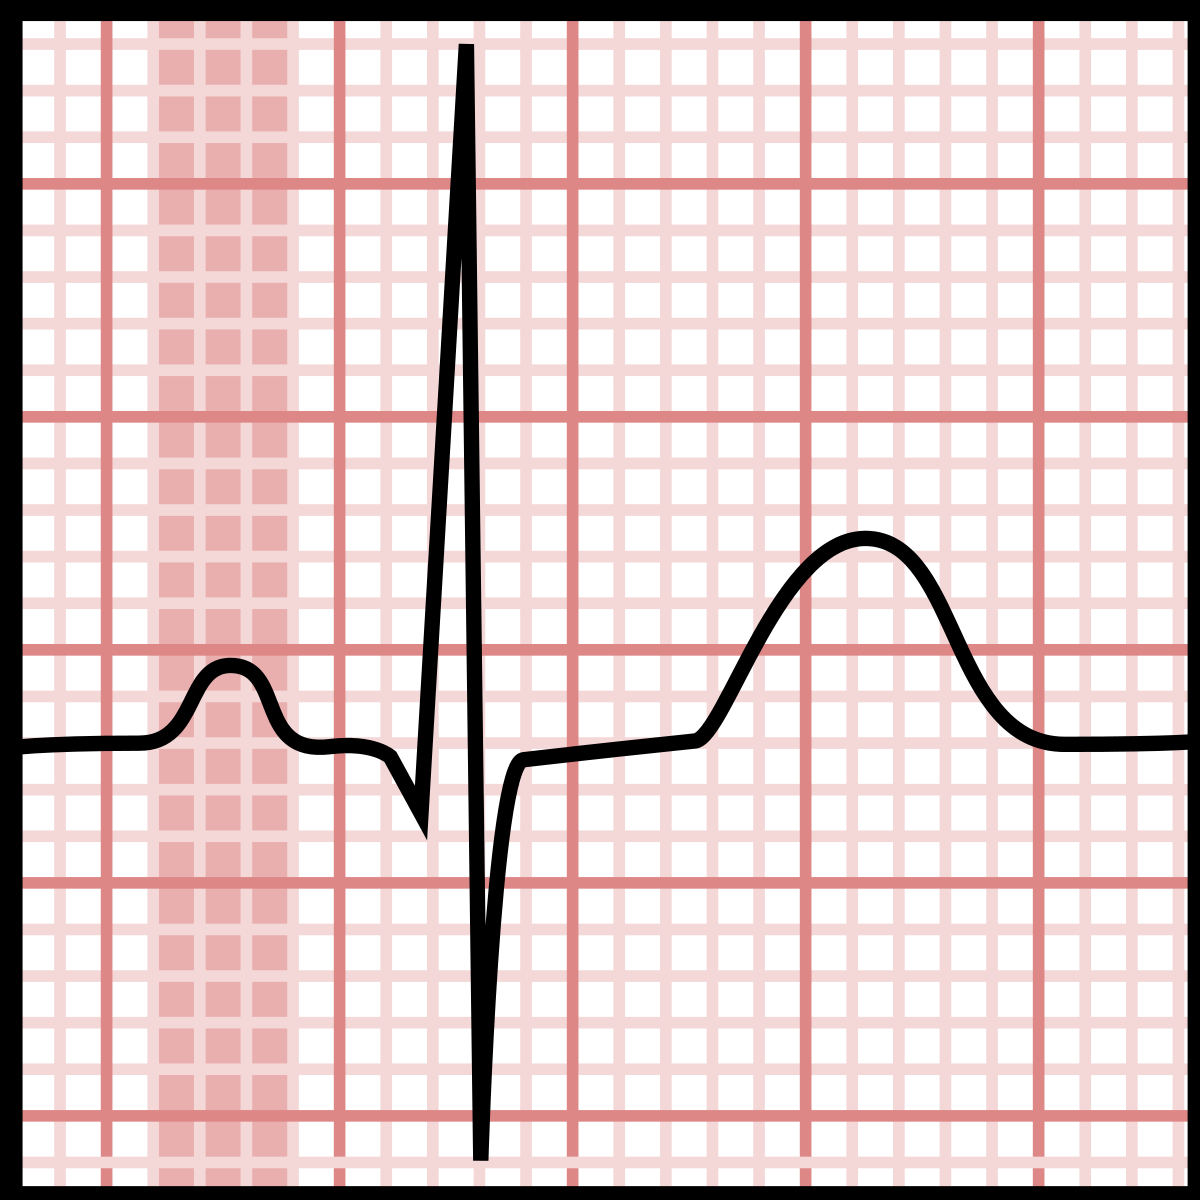
\includegraphics[scale=0.1]{latex_code/Figures_new/p_wave.png}
    \caption{Ρ-κυμάτωση}
    \label{fig:p_wave}
\end{figure}

\begin{figure}[h]
    \centering
    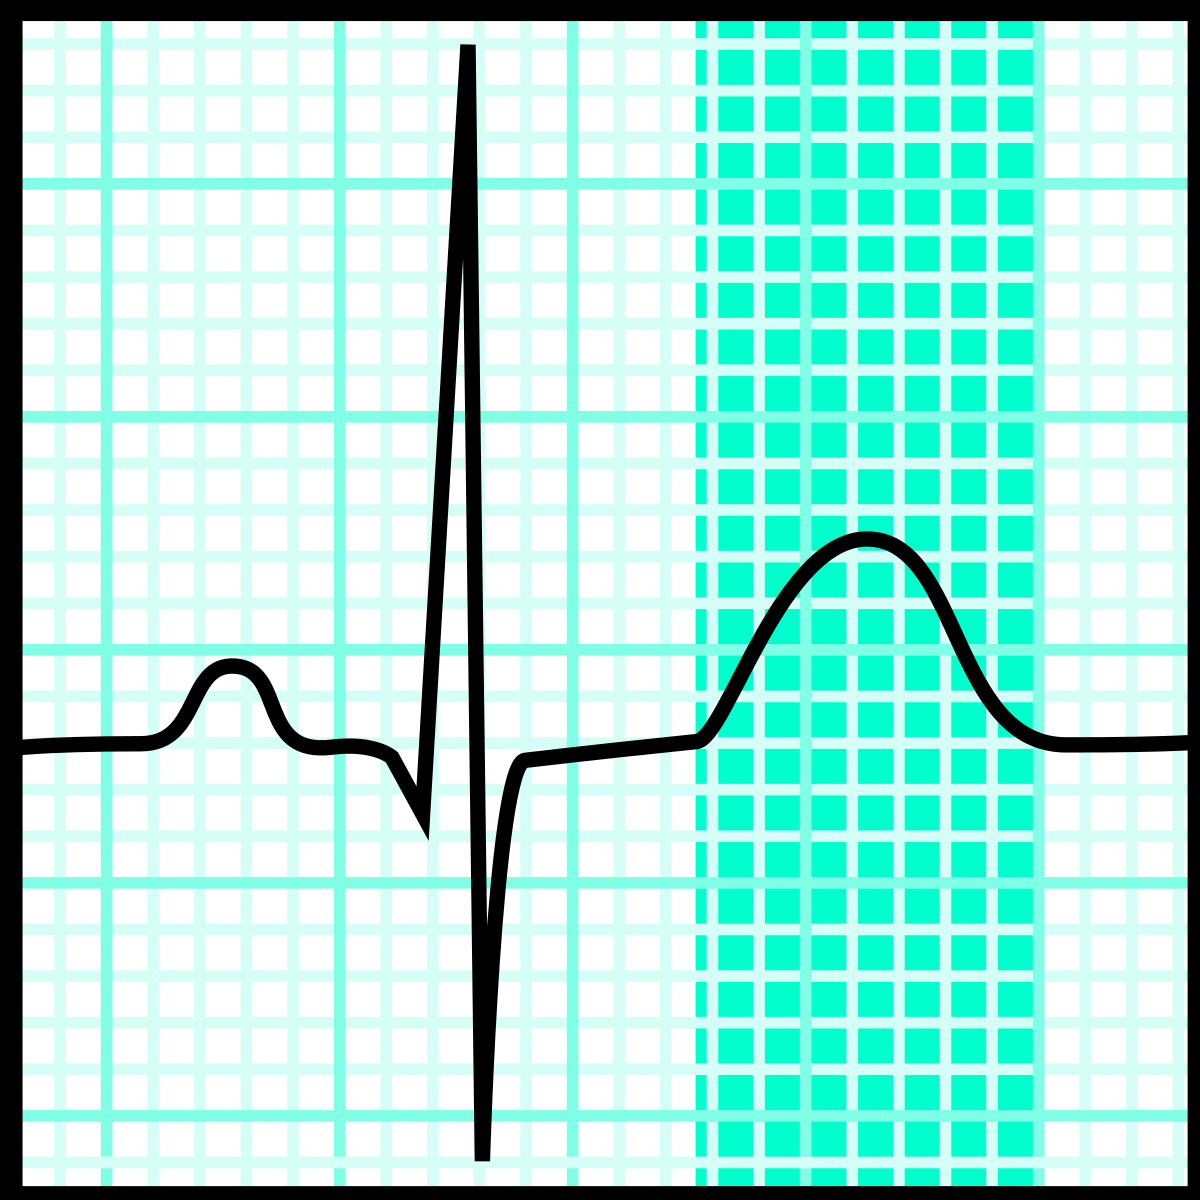
\includegraphics[scale=0.1]{latex_code/Figures_new/t_wave.png}
    \caption{Τ-κυμάτωση}
    \label{fig:t_wave}
\end{figure}

Τα δύο παραπάνω διαστήματα, μας ενδιαφέρουν ιδιαιτέρως, αφενός γιατί η μορφή τους μπορεί να μας δώσει αρκετά χρήσιμα στοιχεία για την αξιολόγηση της φυσιολογικότητας ενός καρδιακού χτύπου, αφετέρου γιατί ενίοτε δημιουργούν προβλήματα στους αλγορίθμους αναγνώρισης των \selectlanguage{english}R\selectlanguage{greek} κορυφών, και συνεπώς χρήζουν ιδιαίτερης σημασίας.

Ανάμεσα στους πολλούς διαθέσιμους αλγόριθμους για τον εντοπισμό των \selectlanguage{english}R\selectlanguage{greek} κορυφών, αποφασίσαμε να χρησιμοποιήσουμε τον αλγόριθμο των \selectlanguage{english}Pan\selectlanguage{greek} και \selectlanguage{english}Tompkins\selectlanguage{greek},\cite{pan_tompkins}, καθώς είναι ένας αλγόριθμος πραγματικού χρόνου, με πολύ καλά αποτελέσματα, μικρές προγραμματιστικές απαιτήσεις και έχει χρησιμοποιηθεί σε πολλές εφαρμογές. Ο αλγόριθμος αυτός δεν χρησιμοποιήθηκε αυτούσιος, αλλά προσαρμόστηκε στα δεδομένα της εφαρμογής.

Στη συνέχεια θα περιγράψουμε τον τρόπο με τον οποίο λειτουργεί ο αλγόριθμος αυτός.


\begin{figure}[h]
    \centering
    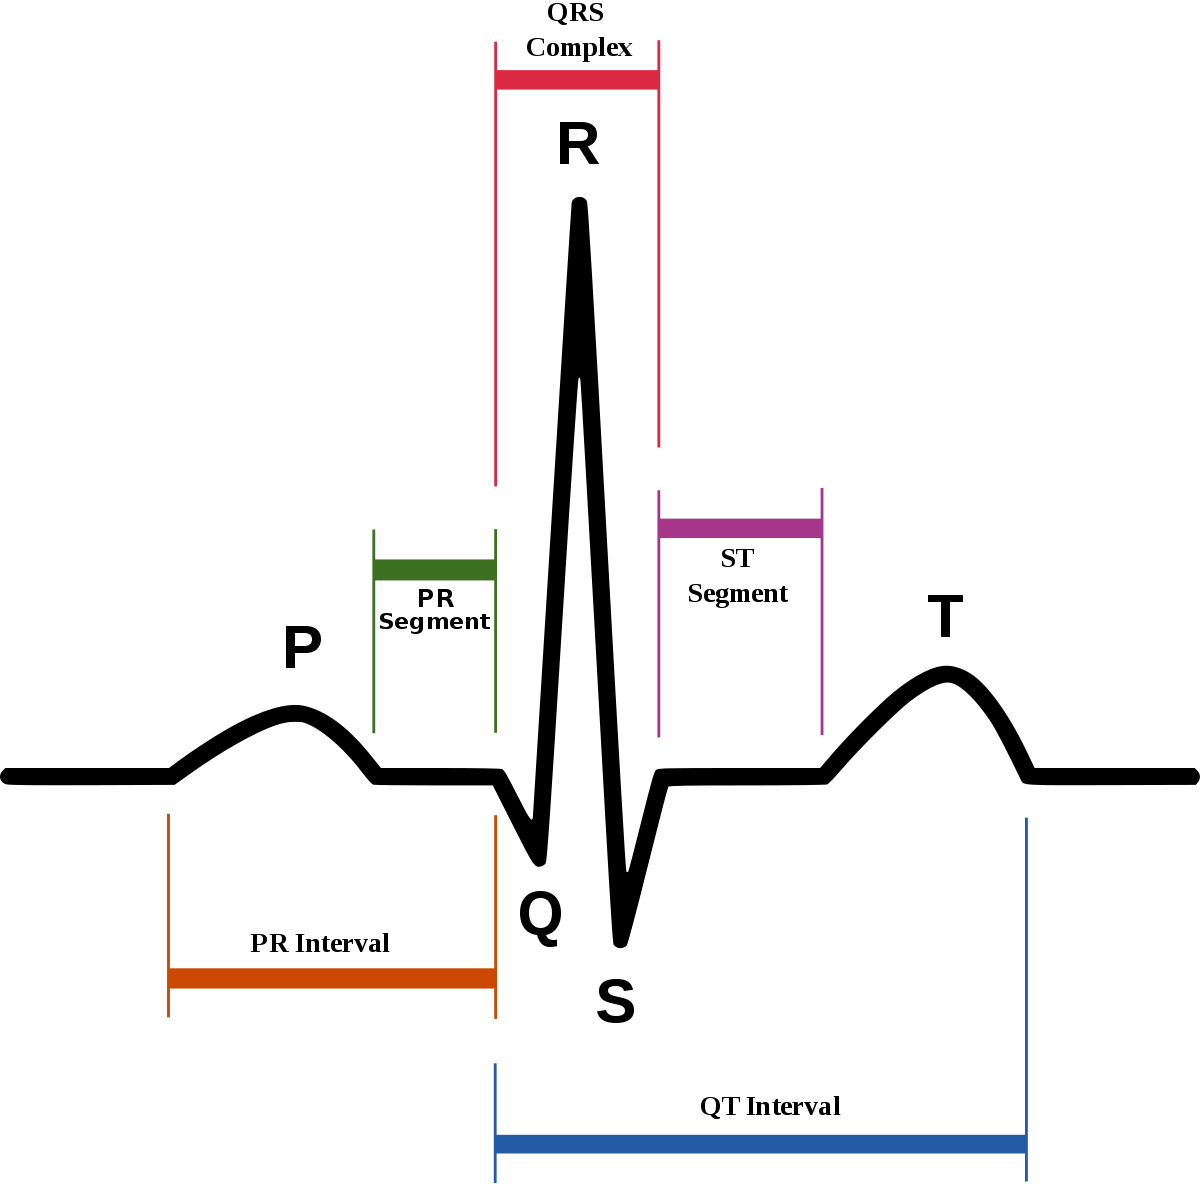
\includegraphics[scale=0.15]{latex_code/Figures_new/qrs.png}
    \caption{Τυπικός διαχωρισμός καρδιακού παλμού σε τμήματα}
    \label{fig:qrs}
\end{figure}

\subsection*{Αλγόριθμος \selectlanguage{english}Pan Tompkins}

\selectlanguage{greek}

\subsubsection*{Εισαγωγικά για τον αλγόριθμο}

Όπως αναφέρθηκε προηγουμένως, ο αλγόριθμος \selectlanguage{english}Pan Tompkins\selectlanguage{greek} είναι ένας αλγόριθμος εντοπισμού κορυφών σε ένα καρδιογράφημα, και είναι πραγματικού χρόνου. Αυτό σημαίνει ότι μπορεί να χρησιμοποιηθεί σε αντίστοιχες εφαρμογές και να δίνει αποτελέσματα την ίδια στιγμή που συμβαίνουν. Ωστόσο, για το πρόβλημα που προσπαθούμε να επιλύσουμε, αυτή η ιδιότητα δεν είναι χρήσιμη, οπότε θα χρησιμοποιήσουμε μια εκδοχή του αλγορίθμου που δεν είναι πραγματικού χρόνου.

Η ανάλυση πραγματικού χρόνου, εισάγει ορισμένους περιορισμούς. Ο πιο σημαντικός εξ αυτών είναι ότι έχουμε να αντιμετωπίσουμε αυστηρά ένα αιτιατό σύστημα. Αντιθέτως, με μια ανάλυση μη πραγματικού χρόνου, μπορούμε να χρησιμοποιήσουμε μη αιτιατά συστήματα, κάτι το οποίο μας επιτρέπει να χρησιμοποιήσουμε "μελοντικές" τιμές μιας κυματομορφής και να εξάγουμε από αυτές χρήσιμη πληροφορία για το "παρόν".

Ένα σημαντικό πλεονέκτημα της παραπάνω ιδιότητας είναι ότι μπορούμε να εφαρμόζουμε ψηφιακά φίλτρα που να εισάγουν μηδενική φάση. Σε αντίθεση με τα \selectlanguage{english}FIR\selectlanguage{greek} φίλτρα \cite{wikiFIR}, που γνωρίζουμε ότι εισάγουν γραμμική φάση αν οι συντελεστές τους είναι συμμετρικοί ως προς το κέντρο τους, τα φίλτρα μηδενικής φάσης δεν εισάγουν καμία φάση, και έτσι μπορούμε να έχουμε το τελικό αποτέλεσμα χωρίς την εισαγωγή καθυστέρησης.

Ο τρόπος με τον οποίο λειτουργούν τα συγκεκριμένα φίλτρα φαίνεται παρακάτω:

\begin{figure}[h]
    \centering
    
\usetikzlibrary{shapes, arrows, positioning}

\selectlanguage{english}

\tikzstyle{block} = [draw, rectangle,
    minimum height=3em, minimum width=4em, align=center, rounded corners = 3pt]
\tikzstyle{sum} = [draw, fill=blue!20, circle, node distance=1cm]
\tikzstyle{input} = [coordinate]
\tikzstyle{output} = [coordinate]
\tikzstyle{pinstyle} = [pin edge={to-,thin,black}]

% The block diagram code is probably more verbose than necessary
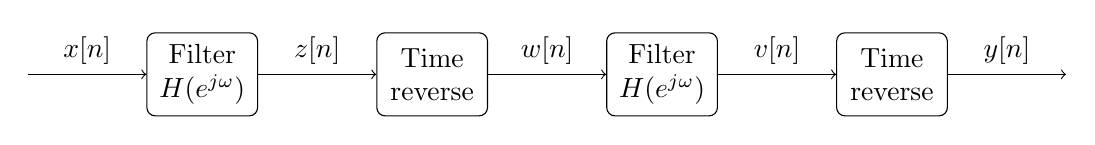
\begin{tikzpicture}[auto]
    % We start by placing the blocks
    \node [input, name=input] {};
    % \node [sum, right of=input] (sum) {};
    \node [block] (band) [right=1.5cm of input] {Filter \\ $H(e^{j\omega})$};
    \node [block] (derivative) [right=1.5 cm of band] {Time \\ reverse};
    \node [block] (squaring) [right=1.5cm of derivative] {Filter \\ $H(e^{j\omega})$};
    \node [block] (moving) [right=1.5cm of squaring] {Time \\ reverse};
    \node [output] (output) [right=1.5cm of moving] {};
    % \node [block, right=of controller, pin={[pinstyle]above:Disturbances},
    %         node distance=3cm] (system) {System of Dawn is the system};
    % We draw an edge between the controller and system block to 
    % calculate the coordinate u. We need it to place the measurement block. 
    % \draw [->] (controller) -- node[name=u] {$u$} (system);
    

    % Once the nodes are placed, connecting them is easy. 
    \draw [draw,->] (input) -- node {$x[n]$} (band);
    \draw [->] (band) -- node {$z[n]$} (derivative);
    \draw [->] (derivative) -- node {$w[n]$} (squaring);
    \draw [->] (squaring) -- node {$v[n]$} (moving);
    \draw [->] (moving) -- node [name=y] {$y[n]$}(output);
    % \draw [->] (moving) |- node {} (derivative);
    % \draw [->] (sum) -- node {$e$} (controller);
    % \draw [->] (moving) -- node [name=y]; {$y$}(output);
    % \draw [->] (y) |- (measurements);
    % \draw [->] (measurements) -| node[pos=0.99] {$-$} 
    %     node [near end] {$y_m$} (sum);
\end{tikzpicture}

\selectlanguage{greek}
    \caption{Διάγραμμα φίλτρων μηδενικής φάσης}
    \selectlanguage{greek}
    \label{fig:zero_phase_fir}
\end{figure}

όπου $z[n] = x[n]*h[n]$, $w[n] = z[-n]$, $v[n] = w[n]*h[n]$ και $y[n] = v[-n]$.
Στο πεδίο της συχνότητας, εύκολα υπολογίζουμε από τα παραπάνω την εξής σχέση:
\begin{equation}
\label{eq:zero_phase_eq}
   Y(e^{j\omega}) = |H(e^{j\omega})|^2X(e^{j\omega})
\end{equation}
Όπως βλέπουμε, η τελική συνάρτηση μεταφοράς έχει θετικούς και πραγματικούς συντελεστές, οπότε επιβεβαιώνεται ότι το παραπάνω φίλτρο εισάγει μηδενική φάση.


\begin{figure}[h]
    \centering
    \selectlanguage{english}

\tikzstyle{block} = [draw, rectangle,
    minimum height=3em, minimum width=4em, align=center, rounded corners = 3pt]
\tikzstyle{sum} = [draw, fill=blue!20, circle, node distance=1cm]
\tikzstyle{input} = [coordinate]
\tikzstyle{output} = [coordinate]
\tikzstyle{pinstyle} = [pin edge={to-,thin,black}]

% The block diagram code is probably more verbose than necessary
\begin{tikzpicture}[auto]
    % We start by placing the blocks
    \node [input, name=input1] {};
    % \node [sum, right of=input] (sum) {};
    \node [block]  (band1) [right=1cm of input1] {Band-pass \\ filtering};
    \node [block] (derivative1) [right=1cm of band1] {Derivative filter};
    \node [block] (squaring1) [right=1cm of derivative1] {Squaring};
    \node [block] (moving1) [right=1cm of squaring1] {Moving window \\integration};
    % \node [block, right=of controller, pin={[pinstyle]above:Disturbances},
    %         node distance=3cm] (system) {System of Dawn is the system};
    % We draw an edge between the controller and system block to 
    % calculate the coordinate u. We need it to place the measurement block. 
    % \draw [->] (controller) -- node[name=u] {$u$} (system);
    \node [output1] [right=1cm of moving1] (output1) {};

    % Once the nodes are placed, connecting them is easy. 
    \draw [draw,->] (input1) -- node {$ECG$} (band1);
    \draw [->] (band1) -- node {} (derivative1);
    \draw [->] (derivative1) -- node {} (squaring1);
    \draw [->] (squaring1) -- node {} (moving1);
    % \draw [->] (moving) -- node [name=y] {$y$}(output);
    % \draw [->] (moving) |- node {} (derivative);
    % \draw [->] (sum) -- node {$e$} (controller);
    % \draw [->] (moving) -- node [name=y]; {$y$}(output);
    % \draw [->] (y) |- (measurements);
    % \draw [->] (measurements) -| node[pos=0.99] {$-$} 
    %     node [near end] {$y_m$} (sum);
\end{tikzpicture}

\selectlanguage{greek}
    \caption{Διάγραμμα των σταδίων προεπεξεργασίας του αλγορίθμου}
    \selectlanguage{greek}
    \label{fig:panTompkins_block}
\end{figure}

\subsubsection*{Ακύρωση θορύβου}
Στο πρώτο βήμα του αλγορίθμου εφαρμόζεται ένα ζωνοπερατό φίλτρο \selectlanguage{english}Butterworth\selectlanguage{greek} \cite{wikiButter} τρίτης τάξης, με συχνότητες αποκοπής τα 5 και 15 \selectlanguage{english}Hz\selectlanguage{greek}. Με την εφαρμογή αυτού του φίλτρου, επιχειρείται να αυξηθεί ο λόγος \selectlanguage{english}SNR\selectlanguage{greek}, καθώς έτσι ελαχιστοποιείται ο μυϊκός θόρυβος, οι ηλεκτρομαγνητικές παρεμβολές στο όργανο μέτρησης, αλλά και οι χαμηλής συχνότητας κυματώσεις.

Για τη συχνότητα δειγματοληψίας καρδιογραφήματος του \selectlanguage{english}Apple Watch\selectlanguage{greek} που είναι ίση με 512.414 \selectlanguage{english}Hz\selectlanguage{greek}, το φίλτρο που προκύπτει είναι το εξής:
\begin{equation}
\label{eq:current_butterworth}
   H_1(z) = 0.0002046\frac{1 -3z^{-2}+3z^{-4}-z^{-6}}{1 - 5.723z^{-1} + 13.680z^{-2}-17.485z^{-3}+12.604z^{-4}-4.859z^{-5}+0.782z^{-6}}
\end{equation}

Σημειώνεται ότι η προγραμματιστική υλοποίηση υπολογίζει αυτόματα τους συντελεστές του φίλτρου 
\selectlanguage{english}Butterworth\selectlanguage{greek} αναλόγως τη συχνότητα. Κατόπιν της εφαρμογής του φίλτρου, η νέα κυματομορφή κανονικοποιείται ως προς τη μέγιστη τιμή που εμφανίζεται σε αυτή. Τα αποτελέσματα του αλγορίθμου εμφανίζονται γραφικά στο σχήμα \ref{fig:pan_tompkins_graph}.

\begin{figure}[h]
    \centering
    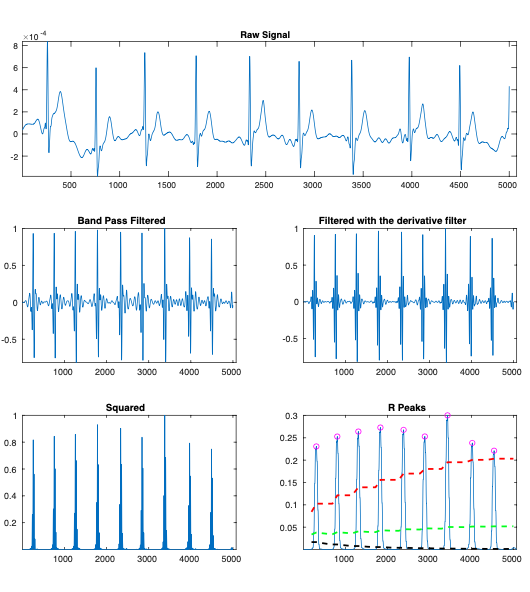
\includegraphics[scale=0.7]{latex_code/Figures_new/graph.png}
    \caption{Στάδια υλοποίησης αλγορίθμου \selectlanguage{english}Pan Tompkins}\selectlanguage{greek}
    \label{fig:pan_tompkins_graph}
\end{figure}

\subsubsection*{Διαφόριση}

Στο δεύτερο στάδιο του αλγορίθμου, εφαρμόζουμε ένα φίλτρο διαφόρισης, έτφσι ώστε να εμφανίζονται πιο έντονες οι γρήγορες εναλλαγές στο σήμα μας. Η αρχική υλοποίηση των \selectlanguage{english}Pan Tompkins\selectlanguage{greek}, για συχνότητα δειγματοληψίας 200 \selectlanguage{english}Hz\selectlanguage{greek}, προτείνει ως φίλτρο διαφόρισης το φίλτρο $H(z) = 0.1(-2z^{-2} - z^{-1} + z^1 +2z^2)$. Στο φίλτρο αυτό όπως βλέπουμε εμφανίζονται δύο διαφορές, η $(z^1-z^{-1})$ και η $2(z^2 - z^{-2})$. 

Αντί αυτού, εμείς θα χρησιμοποιήσουμε την προσαρμοσμένη έκδοση του φίλτρου από τον \selectlanguage{english}Hooman Sedghamiz\selectlanguage{greek} \cite{pan_tompkins_matlab}. Εδώ, το αρχικό φίλτρο που χρησιμοποιείται είναι το φίλτρο $H(z) = (-z^{-3} - 2z^{-2} + 2z^{-1} + 1)$, όπου βλέπουμε πως η μόνη ουσιαστική αλλαγή είναι ότι εναλλάχθηκαν οι συντελεστές των προηγούμενων διαφορών (και μετατοπίστηκαν στο χρόνο ώστε να μπορεί να υλοποιηθεί το φίλτρο χωρίς περαιτέρω επεξεργασία σε υπολογιστή). Συνεπώς, σε μορφή πίνακα, το φίλτρο μας μπορεί να παρασταθεί ως $A = [1, 2, 0, -2, -1]$. (Οι συντελεστές του πίνακα έχουν φθίνοντα αριθμό τάξης)

Χρησιμοποιώντας τον παραπάνω πίνακα, δημιουργούμε έναν καινούργιο πίνακα (και άρα ένα νέο φίλτρο), εφαρμόζοντας γραμμική παρεμβολή στα στοιχεία του πίνακα. Συγκεκριμένα, ξεικνάμε από το πρώτο στοιχείο, και προχωρώντας με βήμα $c = \frac{160}{F_s}$, όπου $F_s$ η συχνότητα δειγματοληψίας, φτάνουμε μέχρι το τελευταίο στοιχείο (χωρίς ωστόσο να το ξεπεράσουμε). Έτσι, ο νέος πίνακας που προκύπτει είναι ο B = [64.1, 84.1, 104.1, 124.1, 96.2, 56.2, 16.2, -23.8, -63.8, -103.8, -120.3, -100.3, -80.3], και το νέο φίλτρο που προκύπτει είναι το 
\begin{equation}
\label{eq:derivation}
   H_2(z) =  \sum_{n=0}^{12}B(n)\cdot z^{-n}
\end{equation}
Μετά από την εφαρμογή της διαφόρισης, το νέο σήμα κανονικοποιείται με τρόπο παρόμοιο με το προηγούμενο βήμα.

\subsubsection*{Ύψωση στο τετράγωνο}

Στο επόμενο βήμα, υψώνουμε το φιλτραρισμένο σήμα στο τετράγωνο. Η ενέργεια αυτή γίνεται για να τονισθούν ακόμη περισσότερο οι κυρίαρχες κορυφές του σήματος, καθώς επίσης και για να μειωθεί η πιθανότητα να αξιολογήσουμε λανθασμένα μια Τ-κυμάτωση ως κορυφή.

\subsubsection*{Ολοκλήρωση - κινούμενος μέσος}

Στο τελευταίο βήμα προεπεξεργασίας του σήματος εφαρμόζουμε μία ολοκλήρωση, ή ένα φίλτρο κινούμενου μέσου στο σήμα μας. Αυτό υλοποιείται με τη συνέλιξη του επεξεργασμένου σήματός μας με ένα σήμα που αποτελείται από μονάδες, και το μήκος του οποίου (μήκος παραθύρου) είναι ίσο με 150 \selectlanguage{english}msec\selectlanguage{greek}, ή $F_s\cdot0.15$ δείγματα. Μέσω αυτής της διαδικασίας, το σήμα μας αποκτά τη μορφή του 5ου διαγράμματος του σχήματος \ref{fig:pan_tompkins_graph}, στο οποίο φαίνεται ότι τα πολλά συμπιεσμένα ακρότατα που υπήρχαν προηγουμένως κοντά στις \selectlanguage{english}R\selectlanguage{greek} κορυφές έχουν αντικατασταθεί πλέον από μία μόνο κορυφή. Η μορφή αυτή του σήματός μας είναι πλεόν κατάλληλη για να εισαχθεί στον τελικό αλγόριθμο εντοπισμού των \selectlanguage{english}R\selectlanguage{greek} κορυφών.

\subsubsection*{Εντοπισμός μεγίστων}

Χρησιμοποιώντας το φιλτραρισμένο σήμα που έχει προκύψει από τα προηγούμενα στάδια επεξεργασίας, εντοπίζουμε όλα τα τοπικά μέγιστα που υπάρχουν στο σήμα μας. Ως τοπικό μέγιστο θεωρούμε κάθε τιμή της κυματομορφής για την οποία το εξεταζόμενο δείγμα είναι μεγαλύτερο από το προηγούμενο και το επόμενο δείγμα. 

Οι \selectlanguage{english}R\selectlanguage{greek} κορυφές του σήματός μας υπάγονται σε έναν σημαντικό περιορισμό εξαιτίας της φυσιολογίας της καρδιάς. Συγκεκριμένα, δεν μπορούν να απέχουν μεταξύ τους λιγότερο από 200 \selectlanguage{english}msec\selectlanguage{greek}, καθώς αυτή είναι η ελάχιστη περίοδος ανάκαμψης της καρδιάς (Τ-κυμάτωση) \cite{wikiT_wave}. 

Συνεπώς, ελέγχουμε τα μέγιστα σημεία που έχουμε βρει, και από όσα απέχουν μεταξύ τους λιγότερο από 200 \selectlanguage{english}msec\selectlanguage{greek} κρατάμε μόνο αυτά που έχουν την υψηλότερη τιμή (δηλαδή αυτά που έχουν τη μεγαλύτερη πιθανότητα να είναι όντως \selectlanguage{english}R\selectlanguage{greek} κορυφές).

\subsubsection*{Κατώφλια}


\subsection{Εξαγωγή χαρακτηριστικών}

Τα χαρακτηριστικά που εξήχθησαν, εννοιολογικά, χωρίζονται στις εξής τρεις κατηγορίες:
\begin{itemize}
    \item Χαρακτηριστικά στο πεδίο του χρόνου
    \item Χαρακτηριστικά στο πεδίο της συχνότητας
    \item Μη γραμμικά χαρακτηριστικά
\end{itemize}

Στη συνέχεια θα αναλύσουμε την κάθε κατηγορία ξεχωριστά και θα παρουσιάσουμε αναλυτικά όλα τα εξαγόμενα χαρακτηριστικά.

\subsubsection*{Ορισμός συνήθων μαθηματικών μεγεθών και στατιστικών μέτρων}
Παρακάτω ορίζονται μερικά συνήθη μαθηματικά μεγέθη και στατιστικά μέτρα που χρησιμοποιήθηκαν στην ανάλυσή μας.
\paragraph{Δειγματική μέση τιμή}
Η δειγματική μέση τιμή ενός μεγέθους \selectlanguage{english}x\selectlanguage{greek} ορίζεται ως εξής:
\begin{equation}
\label{eq:mean}
   \overline{x}=\frac{\sum_{j=1}^{N} x_j}{N}
\end{equation}
όπου \selectlanguage{english}$x_j$\selectlanguage{greek} μια παρατήρηση του μεγέθους, και Ν το πλήθος των παρατηρήσεων. Η δειγματική μέση τιμή, ή απλά μέση τιμή ενός μεγέθους \selectlanguage{english}x\selectlanguage{greek} θα συμβολίζεται ως \selectlanguage{english}$\overline{x}$\selectlanguage{greek}, ή ως $E(x)$.

\paragraph{Τυπική απόκλιση}
Η τυπική απόκλιση ενός μεγέθους \selectlanguage{english}x\selectlanguage{greek} ορίζεται ως εξής:
\begin{equation}
\label{eq:standard_deviation}
   \sigma(x)=\sqrt{\frac{\sum_{j=1}^{N} |x_j-\overline{x}|^2 }{N-1}}
\end{equation}
όπου \selectlanguage{english}$x_j$\selectlanguage{greek} μια παρατήρηση του μεγέθους, και Ν το πλήθος των παρατηρήσεων. Η τυπική απόκλιση ενός μεγέθους \selectlanguage{english}x\selectlanguage{greek} θα συμβολίζεται ως \selectlanguage{english}$\sigma(x)$\selectlanguage{greek}.


\paragraph{\selectlanguage{english}R-R\selectlanguage{greek} διάστημα}
Ως \selectlanguage{english}R-R\selectlanguage{greek} διάστημα, ορίζουμε τη χρονική διαφορά
\begin{equation}
\label{eq:RR}
   RR_i = t(R_{i+1}) - t(R_i)
\end{equation}
όπου \selectlanguage{english}$t(R_i)$\selectlanguage{greek} η χρονική στιγμή που συμβαίνει ο χτύπος (\selectlanguage{english}R\selectlanguage{greek} σημείο) \selectlanguage{english}i\selectlanguage{greek}. Το \selectlanguage{english}R-R\selectlanguage{greek} διάστημα, που ουσιαστικά μετράει τη διάρκεια μεταξύ δύο διαδοχικών καρδιακών χτύπων, θα μετριέται κατά σύμβαση σε χιλιοστά του δευτερολέπτου, και θα συμβολίζεται ως \selectlanguage{english}$RR_i$\selectlanguage{greek}.


\paragraph{Ν-Ν διάστημα}
Το σύνολο των Ν-Ν διαστημάτων είναι ένα υποσύνολο των \selectlanguage{english}R-R\selectlanguage{greek} διαστημάτων. Τόσο το \selectlanguage{english}R-R\selectlanguage{greek} σύνολο, όσο και το Ν-Ν είναι διατεταγμένα σύνολα, δηλαδή η σειρά με την οποία έρχονται τα στοιχεία τους έχει σημασία. Προγραμματιστικά, υλοποιούνται με τη χρήση μιας απλής λίστας, ή ενός μονοδιάστατου πίνακα. Το σύνολο Ν-Ν δημιουργείται από τον εξής αλγόριθμο:
\begin{enumerate}
    \item Αρχικά το σύνολο Ν-Ν είναι ένα κενό σύνολο.
    \item Δημιουργείται μια κενή "ουρά" τεσσάρων θέσεων, την οποία θα ονομάζουμε ουρά σύγκρισης (ΟΣ). Με τον όρο "ουρά", εννοούμε μια δομή δεδομένων \selectlanguage{english}First In First Out\selectlanguage{greek}. Η μέση τιμή των στοιχείων της ουράς συμβολίζεται ως $\overline{O\Sigma}$.
    \item Η ΟΣ γεμίζει για πρώτη φορά, με τρόπο που θα αναλύσουμε πιο κάτω από τον βασικό αλγόριθμο, για λόγους ευκολίας ανάγνωσης.
    \item Για κάθε στοιχείο $RR_i$ του \selectlanguage{english}R-R\selectlanguage{greek} πίνακα κάνουμε τα εξής:
    \begin{enumerate}
        \item Αν $ 0.85 \cdot \overline{O\Sigma} \le RR_i \le 1.15 \cdot \overline{O\Sigma} $, προσθέτουμε την $RR_i$ στο τέλος του πίνακα των Ν-Ν, και εισάγουμε το στοιχείο αυτό στην ΟΣ.
        \item Αλλιώς, εάν $ 0.75 \cdot \overline{O\Sigma} \le RR_i \le 1.25 \cdot \overline{O\Sigma} $, εισάγουμε το στοιχείο στην ΟΣ.
    \end{enumerate}
\end{enumerate}
Για την αρχικοποίηση της ΟΣ, δημιουρηούμε έναν κινούμενο μέσο (ΚΜ) 8 στοιχείων, δηλαδή παίρνουμε την μέση τιμή των 8 πρώτων στοιχείων. Μέχρι να γεμίσει η ΟΣ, ελέγχουμε εάν $ 0.75 \cdot KM \le RR_i \le 1.25 \cdot KM $, και σε περίπτωση που αυτό ισχύει, προσθέτουμε το $RR_i$ στοιχείο στην ΟΣ. Στη συνέχεια, ανανεώνουμε τον ΚΜ ξεκινώντας από το επόμενο στοιχείο και επαναλαμβάνουμε μέχρι να πληροίται η συνθήκη τερματισμού.

Μια ερμηνεία των Ν-Ν διαστημάτων είναι ότι πρόκειται για τα "φυσιολογικά" διαστήματα σε ένα καρδιογράφημα, εννοώντας τα διαστήματα που δεν έχουν πολύ σημαντικές διαφορές στη χρονική τους διάρκεια σε σύγκριση με τα γειτονικά τους. Καθώς οι κορυφές των καρδιακών χτύπων εντοπίζονται αλγοριθμικά, ορισμένες φορές ο αλγόριθμος μπορεί να οδηγήσει σε λανθασμένα αποτελέσματα, που με τη σειρά τους μπορούν να οδηγήσουν σε έντονες μεταβολές στη διάρκεια των \selectlanguage{english}R-R\selectlanguage{greek} διαστημάτων. Χρησιμποιώντας το σύνολο Ν-Ν, το πρόβλημα αυτό περιορίζεται σημαντικά.

Ο παραπάνω αλγόριθμος, διασφαλίζει ένα ποσοστιαίο όριο απόκλισης του κάθε διαστήματος από τα γειτονικά του. Όταν ξεπερνιέται το όριο αυτό, το παρόν διάστημα δεν αξιολογείται ως φυσιολογικό. Πέρα από αυτό όμως, υπάρχει ένα ακόμα όριο, περισσότερο ελαστικό, που καθορίζει εάν το παρόν διάστημα θα χρησιμοποιηθεί ως διάστημα σύγκρισης για τα επόμενα. Ο λόγος που υφίσταται το όριο αυτό και είναι πιο ελαστικό, είναι για να αποφεύγονται καταστάσεις αστάθειας στο σύστημα. Ο αλγόριθμος αυτός είναι μια προσαρμογή του αλγόριθμου των Barbara Mali κ.α. \cite{barbara_mali_alg}

\subsubsection{Χαρακτηριστικά στο πεδίο του χρόνου}

Τα χαρακτηριστικά στο πεδίο του χρόνου ποσοτικοποιούν το μέγεθος της διακύμανσης του καρδιακού ρυθμού, και, ως επί τω πλείστω, είναι στατιστικές μετρικές που σχετίζονται άμεσα με το παρατηρούμενο μέγεθος (ΔΚΡ). Παρακάτω, παρουσιάζονται αναλυτικά.


\paragraph{\selectlanguage{english}SDRR\selectlanguage{greek}}
\selectlanguage{greek}
Η μετρική \selectlanguage{english}SDRR (Standard Deviation of R-R Intervals) \selectlanguage{greek}είναι η τυπική απόκλιση όλων των διαστημάτων  \selectlanguage{english}R-R\selectlanguage{greek}. Δίνεται από τον τύπο
\begin{equation}
\label{eq:SDRR}
   SDRR=\sigma(RR_i)
\end{equation}
Υπολογίζεται σε χιλιοστά του δευτερολέπτου.

\paragraph{\selectlanguage{english}AHR\selectlanguage{greek}}
Η μετρική \selectlanguage{english}AHR (Average Heart Rate) \selectlanguage{greek}εκφράζει τους μέσους χτύπους ανά λεπτό. Δίνεται από τον τύπο
\begin{equation}
\label{eq:AHR}
   AHR=\frac{60}{\overline{RR_i}}
\end{equation}
Υπολογίζεται σε χτύπους ανά λεπτό.

\paragraph{\selectlanguage{english}SDNN\selectlanguage{greek}}
Η μετρική \selectlanguage{english}SDNN (Standard Deviation of N-N Intervals)  \selectlanguage{greek}ποσοτικοποιεί την τυπική απόκλιση των Ν-Ν διαστημάτων. Δίνεται από τον τύπο
\begin{equation}
\label{eq:SDRR}
   SDNN=\sigma(NN_i)
\end{equation}
Υπολογίζεται σε χιλιοστά του δευτερολέπτου.

\paragraph{\selectlanguage{english}SDSD\selectlanguage{greek}}
Η μετρική \selectlanguage{english}SDSD (Standard Deviation of Successive Differences)  \selectlanguage{greek}ποσοτικοποιεί την τυπική απόκλιση μεταξύ των διαφορών των διακρειών δύο γειτονικών Ν-Ν διαστημάτων. Δίνεται από τον τύπο
\begin{equation}
\label{eq:SDRR}
   SDSD=\sigma(|NN_{i+1} - NN_i|)
\end{equation}
Υπολογίζεται σε χιλιοστά του δευτερολέπτου.

\paragraph{\selectlanguage{english}SDANN\selectlanguage{greek}}
Η μετρική \selectlanguage{english}SDANN (Standard Deviation of Average N-N Intervals on Ultra Short Intervals)  \selectlanguage{greek} εκφράζει την τυπική απόκλιση μεταξύ των μέσων τιμών των διαρκειών των Ν-Ν διαστημάτων, σε κάθε υποδιάστημα των 30 δευτερολέπτων του συνολικού δείγματος (διάρκειας 5 λεπτών).

Ουσιαστικά, χωρίζουμε το κάθε δείγμα σε 10 διαστήματα των 30 δευτερολέπτων, υπολογίζουμε τη μέση τιμή διάρκειας του Ν-Ν διαστήματος για κάθε ένα από τα 10 διαστήματα, και τέλος λαμβάνουμε την τυπική απόκλιση αυτών των 10 τιμών. Δίνεται από τον τύπο
\begin{equation}
\label{eq:SDANN}
   SDANN=\sigma(E((NN_i)_{UST}))
\end{equation}

Με τον όρο \selectlanguage{english}"UST"\selectlanguage{greek} εννοούμε το κάθε διάστημα πολύ μικρής διάρκειας. Υπολογίζεται σε χιλιοστά του δευτερολέπτου.

\paragraph{\selectlanguage{english}SDNNI\selectlanguage{greek}}
Η μετρική \selectlanguage{english}SDNNI (Mean of Standard Deviations of N-N Intervals on Ultra Short Intervals)  \selectlanguage{greek} εκφράζει τη μέση τιμή μεταξύ των τυπικών αποκλίσεων των διαρκειών των Ν-Ν διαστημάτων, σε κάθε υποδιάστημα των 30 δευτερολέπτων του συνολικού δείγματος (διάρκειας 5 λεπτών).

Ουσιαστικά, χωρίζουμε το κάθε δείγμα σε 10 διαστήματα των 30 δευτερολέπτων, υπολογίζουμε την τυπική απόκλιση διάρκειας του Ν-Ν διαστήματος για κάθε ένα από τα 10 διαστήματα, και τέλος λαμβάνουμε τη μέση τιμή αυτών των 10 τιμών. Δίνεται από τον τύπο
\begin{equation}
\label{eq:SDNNI}
   SDNNI=E((\sigma(NN_i)_{UST}))
\end{equation}

Με τον όρο \selectlanguage{english}"UST"\selectlanguage{greek} εννοούμε το κάθε διάστημα πολύ μικρής διάρκειας. Υπολογίζεται σε χιλιοστά του δευτερολέπτου.

\paragraph{\selectlanguage{english}pNN50\selectlanguage{greek}}
Η μετρική \selectlanguage{english}pNN50 (Percentage of Adjacent N-N intervals With More Than 50 msec Difference)  \selectlanguage{greek} εκφράζει το ποσοστό των γειτονικών διαστημάτων Ν-Ν που έχουν μεγαλύτερη διαφορά μεταξύ τους από 50 \selectlanguage{english}msec.\selectlanguage{greek}

\paragraph{\selectlanguage{english}RMSSD\selectlanguage{greek}}
Η μετρική \selectlanguage{english}RMSSD (Root Mean Square of Successive Differences)\selectlanguage{greek} δίνεται από τον τύπο 
\begin{equation}
\label{eq:RMSSD}
   RMSSD = \sqrt{\frac{1}{N-1}\cdot\sum_{j=1}^N(NN_j)^2}
\end{equation}
όπου Ν είναι το πλήθος των παρατηρήσεων. Υπολογίζεται σε χιλιοστά του δευτερολέπτου.

\paragraph{\selectlanguage{english}HTI\selectlanguage{greek}}
Η μετρική \selectlanguage{english}HTI (Heart Rate Variability Triangular Index)\selectlanguage{greek} είναι μια γεωμετρική ερμηνεία που προκύπτει από τη ΔΚΡ. Υπολογίζεται ως εξής:
\begin{enumerate}
    \item Δημιουργούμε ένα ιστόγραμμα με τις διάρκειες των Ν-Ν διαστημάτων, και το πλήθος των διαστημάτων που έχουν αυτή τη διάρκεια. Το βήμα, ή η διακριτικότητα των διαστημάτων αυτών είναι ο ακέραιος αριθμός που βρίσκεται πιο κοντά στα 8 χιλιοστά του δευτερολέπτου. Για παράδειγμα, ένα διάστημα με διάρκεια 720 χιλιοστά και συχνότητα δειγματοληψίας 125 \selectlanguage{english}Hz\selectlanguage{greek} θα έχει διακριτική ικανότητα ένα δείγμα, και άρα το παραπάνω διάστημα θα εισαχθεί στο ιστόγραμμα με την τιμή 90.
    \item Μόλις ολοκληρωθεί η παραπάνω διαδικασία, βρίσκουμε την μπάρα του ιστογράμματος με το μεγαλύτερο ύψος, δηλαδή την πιο συχνή διάρκεια που εμφανίζεται στα διαστήματά μας.
    \item Το τελικό μας αποτέσμα προκύπτει από τη διαίρεση της παραπάνω τιμής με το πλήθος των διαφορετικών μπάρων που υπάρχουν.
\end{enumerate}

\paragraph{\selectlanguage{english}HRmaxmin\selectlanguage{greek}}
Η μετρική \selectlanguage{english}HRmaxmin (Heart Rate Maximum - Heart Rate Minimum)\selectlanguage{greek} εκφράζει τη διαφορά μεταξύ μέγιστου και ελάχιστου καρδιακού ρυθμού. Δίνεται από τη σχέση
\begin{equation}
\label{eq:hrmaxmin}
   HRmaxmin = \frac{60}{min(NN_i)} - \frac{60}{max(NN_i)}
\end{equation}
Υπολογίζεται σε χτύπους ανά λεπτό.

\subsubsection{Χαρακτηριστικά στο πεδίο της συχνότητας}
Για την εξαγωγή των συχνοτικών χαρακτηριστικών, απαραίτητο προστάδιο είναι η μετατροπή των δειγμάτων μας σε ένα συχνοτικό πεδίο. Στην παρούσα μελέτη, αυτό έγινε με τη χρήση του διακριτού μετασχηματισμού \selectlanguage{english}Fourier\selectlanguage{greek}\cite{wikiDFT}, και συγκεκριμένα με τη χρήση του αλγορίθμου \selectlanguage{english}Fast Fourier Transform.\selectlanguage{greek} \cite{wikiFFT} Ο παραπάνω αλγόριθμος, είναι αλγόριθμος με πολυπλοκότητα \selectlanguage{english}O(NlogN)\selectlanguage{greek}, συνεπώς έχει μικρό κόστος προγραμματιστικά και ενδείκνυται για αναλύσεις πραγματικού χρόνου.

Η διακριτική ικανότητα στον αξόνα των συχνοτήτων ως γνωστόν είναι ίση με τον αντίστροφο αριθμό της διάρκειας του δείγματος. Στην προκειμένη περίπτωση λοιπόν, με τα δείγματα να έχουν διάρκεια 5 λεπτά, η διακριτική ικανότητα στη συχνότητα είναι 0.0033 \selectlanguage{english}Hz.\selectlanguage{greek}

Παρακάτω, παρουσιάζονται τα συχνοτικά χαρακτηριστικά που εξήχθησαν.


\paragraph{\selectlanguage{english}VLFBE\selectlanguage{greek}}
Η μετρική \selectlanguage{english}VLFBE (Very Low Frequency Band Energy)\selectlanguage{greek} εκφράζει το σύνολο της ενέργειας που υπάρχει στο φάσμα των πολύ χαμηλών συχνοτήτων. Οι πολύ χαμηλές συχνότητες, ορίζονται ως $F_{VLF} = [0.0033, 0.04]$ \selectlanguage{english}Hz\selectlanguage{greek}. Συνεπώς, η ενέργεια πολύ χαμηλών συχνοτήτων δίνεται από τον τύπο
\begin{equation}
\label{eq:vlfbe}
   VLFBE = \sum_{i=0.0033}^{0.04}f_i^2
\end{equation}
όπου το στοιχείο $i$ είναι πολλαπλάσιο του $1/300$, και $f_i$ το στοιχείο με θέση $i$ της μετασχηματισμένης κάτα $FFT$ κυματομορφής του δείγματος. Μετριέται σε $s^2$.

\paragraph{\selectlanguage{english}VLFBEP\selectlanguage{greek}}
Η μετρική \selectlanguage{english}VLFBEP (Very Low Frequency Band Energy Percentage)\selectlanguage{greek} εκφράζει το ποσοστό της ενέργειας που υπάρχει στο φάσμα των πολύ χαμηλών συχνοτήτων, σε σχέση με το σύνολο της ενέργειας. Το ποσοστό της ενέργειας πολύ χαμηλών συχνοτήτων, δίνεται από τον τύπο
\begin{equation}
\label{eq:vlfbep}
   VLFBEP = \frac{VLFBE}{\sum{f_i^2}}
\end{equation}
όπου το στοιχείο άθροισμα του παρονομαστή αφορά όλα τα στοιχεία του δείγματος.

\paragraph{\selectlanguage{english}VLFP\selectlanguage{greek}}
Η μετρική \selectlanguage{english}VLFP (Very Low Frequency Peak)\selectlanguage{greek} εκφράζει τη συγκεκριμένη συχνότητα που ανήκει στις πολύ χαμηλές συχνότητες και για την οποία έχουμε τη μέγιστη ενέργεια. Υπολογίζεται σε $Hz$.


\paragraph{\selectlanguage{english}LFBE\selectlanguage{greek}}
Η μετρική \selectlanguage{english}LFBE (Low Frequency Band Energy)\selectlanguage{greek} εκφράζει το σύνολο της ενέργειας που υπάρχει στο φάσμα των χαμηλών συχνοτήτων. Οι χαμηλές συχνότητες, ορίζονται ως $F_{LF} = (0.04, 0.15]$ \selectlanguage{english}Hz\selectlanguage{greek}. Συνεπώς, η ενέργεια χαμηλών συχνοτήτων δίνεται από τον τύπο
\begin{equation}
\label{eq:lfbe}
   LFBE = \sum_{i=0.0433}^{0.15}f_i^2
\end{equation}
όπου το στοιχείο $i$ είναι πολλαπλάσιο του $1/300$, και $f_i$ το στοιχείο με θέση $i$ της μετασχηματισμένης κάτα $FFT$ κυματομορφής του δείγματος. Μετριέται σε $s^2$.

\paragraph{\selectlanguage{english}LFBEP\selectlanguage{greek}}
Η μετρική \selectlanguage{english}LFBEP (Low Frequency Band Energy Percentage)\selectlanguage{greek} εκφράζει το ποσοστό της ενέργειας που υπάρχει στο φάσμα των χαμηλών συχνοτήτων, σε σχέση με το σύνολο της ενέργειας. Το ποσοστό της ενέργειας χαμηλών συχνοτήτων, δίνεται από τον τύπο
\begin{equation}
\label{eq:lfbep}
   LFBEP = \frac{LFBE}{\sum{f_i^2}}
\end{equation}
όπου το στοιχείο άθροισμα του παρονομαστή αφορά όλα τα στοιχεία του δείγματος.

\paragraph{\selectlanguage{english}LFP\selectlanguage{greek}}
Η μετρική \selectlanguage{english}LFP (Low Frequency Peak)\selectlanguage{greek} εκφράζει τη συγκεκριμένη συχνότητα που ανήκει στις χαμηλές συχνότητες και για την οποία έχουμε τη μέγιστη ενέργεια. Υπολογίζεται σε $Hz$.


\paragraph{\selectlanguage{english}HFBE\selectlanguage{greek}}
Η μετρική \selectlanguage{english}HFBE (High Frequency Band Energy)\selectlanguage{greek} εκφράζει το σύνολο της ενέργειας που υπάρχει στο φάσμα των υψηλών συχνοτήτων. Οι υψηλές συχνότητες, ορίζονται ως $F_{HF} = (0.15, 0.4]$ \selectlanguage{english}Hz\selectlanguage{greek}. Συνεπώς, η ενέργεια υψηλών συχνοτήτων δίνεται από τον τύπο
\begin{equation}
\label{eq:hfbe}
   HFBE = \sum_{i=0.1533}^{0.4}f_i^2
\end{equation}
όπου το στοιχείο $i$ είναι πολλαπλάσιο του $1/300$, και $f_i$ το στοιχείο με θέση $i$ της μετασχηματισμένης κάτα $FFT$ κυματομορφής του δείγματος. Μετριέται σε $s^2$.

\paragraph{\selectlanguage{english}HFBEP\selectlanguage{greek}}
Η μετρική \selectlanguage{english}HFBEP (High Frequency Band Energy Percentage)\selectlanguage{greek} εκφράζει το ποσοστό της ενέργειας που υπάρχει στο φάσμα των υψηλών συχνοτήτων, σε σχέση με το σύνολο της ενέργειας. Το ποσοστό της ενέργειας υψηλών συχνοτήτων, δίνεται από τον τύπο
\begin{equation}
\label{eq:hfbep}
   HFBEP = \frac{HFBE}{\sum{f_i^2}}
\end{equation}
όπου το στοιχείο άθροισμα του παρονομαστή αφορά όλα τα στοιχεία του δείγματος.

\paragraph{\selectlanguage{english}HFP\selectlanguage{greek}}
Η μετρική \selectlanguage{english}HFP (High Frequency Peak)\selectlanguage{greek} εκφράζει τη συγκεκριμένη συχνότητα που ανήκει στις υψηλές συχνότητες και για την οποία έχουμε τη μέγιστη ενέργεια. Υπολογίζεται σε $Hz$.

\paragraph{\selectlanguage{english}LF/HF\selectlanguage{greek}}
Η μετρική \selectlanguage{english}LF/HF (Low Frequency to High Frequency Ratio)\selectlanguage{greek} υπολογίζει το λόγο της ενέργειας χαμηλών συχνοτήτων, προς την ενέργεια υψηλών συχνοτήτων.